\documentclass[aspectratio=169]{beamer}
% \usepackage{pgfpages}
% \pgfpagesuselayout{4 on 1}[a4paper,landscape,border shrink=5mm]
\usepackage{tikz}
\usetikzlibrary{shapes, backgrounds, arrows, positioning}
%\usepackage{pgfplots}
\usepackage{listings}
\usepackage[utf8,latin1]{inputenc}
\usepackage[natbibapa]{apacite}

\makeatletter \def\newblock{\beamer@newblock} \makeatother  

\beamertemplatenavigationsymbolsempty
\setbeamertemplate{itemize items}[circle]
\setbeamertemplate{section in toc}[circle]
% \mode<beamer>{\setbeamercolor{math text displayed}{fg=iwmgray}}
\setbeamercolor{block body}{bg=iwmorange!50!white}
\setbeamercolor{block title}{fg=white, bg=iwmorange}

% Definitions for biblatex
\setbeamercolor{bibliography entry note}{fg=iwmgray}
\setbeamercolor{bibliography entry author}{fg=iwmgray}
\setbeamertemplate{bibliography item}{}

\definecolor{iwmorange}{RGB}{255,105,0}
\definecolor{iwmgray}{RGB}{67,79,79}
\definecolor{iwmblue}{RGB}{60,180,220}
\definecolor{iwmgreen}{RGB}{145,200,110}
\definecolor{iwmpurple}{RGB}{120,0,75}

\definecolor{beamerblue}{rgb}{0.2,0.2,0.7}

% \setbeamercolor{title}{fg=iwmorange}
% \setbeamercolor{frametitle}{fg=iwmorange}
% \setbeamercolor{structure}{fg=iwmorange}
% \setbeamercolor{normal text}{fg=iwmgray}
% \setbeamercolor{author}{fg=iwmgray}
% \setbeamercolor{date}{fg=iwmgray}

\title{Power simulation for mixed-effects models}
%\author{Nora Wickelmaier}

\date{Last modified: 2025-03-26}

\newcommand{\vect}[1]{\mathbf{#1}}
\newcommand{\mat}[1]{\mathbf{#1}}
\newcommand{\gvect}[1]{\boldsymbol{#1}}
\newcommand{\gmat}[1]{\boldsymbol{#1}}

\lstset{language = R,%
  basicstyle = \ttfamily\color{iwmgray},
  frame = single,
  rulecolor = \color{iwmgray},
  commentstyle = \slshape\color{iwmgreen},
  keywordstyle = \bfseries\color{iwmgray},
  identifierstyle = \color{iwmpurple},
  stringstyle = \color{iwmblue},
  numbers = none,%left,numberstyle = \tiny,
  basewidth = {.5em, .4em},
  showstringspaces = false,
  emphstyle = \color{red!50!white}}

\AtBeginSection[]{
  \frame{
    \tableofcontents[sectionstyle=show/hide, subsectionstyle=show/show/hide]}}

\setbeamertemplate{headline}{
 \begin{beamercolorbox}{section in head}
   \vskip5pt\insertsectionnavigationhorizontal{\paperwidth}{}{}\vskip2pt
 \end{beamercolorbox}
}

\setbeamertemplate{footline}{\vskip-2pt\hfill\insertframenumber$\;$\vskip2pt}

\begin{document}

\begin{frame}{}
\thispagestyle{empty}
\titlepage
\end{frame}

\begin{frame}{Outline}
\tableofcontents
\end{frame}

\section[Introduction]{Introduction mixed-effects models}

% \begin{frame}{Mixed-effects models}
% \begin{itemize}
%   \item Mixed-effects models take account of dependencies in hierarchical,
%     longitudinal, and other dependent data
%   \item Mixed-effects models have been developed in a variety of
%     disciplines with varying names and terminology
%   \begin{itemize}
%     \item Random-effects models (statistics, econometrics)
%     \item Variance and covariance component analysis (statistics)
%     \item Hierarchical linear models (education)
%     \item Multilevel models (sociology)
%     \item Contextual-effects models (sociology, political science)
%     \item Random-coefficient models (econometrics)
%     \item Repeated-measures models (statistics, psychology)
%   \end{itemize}
% \end{itemize}
%   \begin{flushright}{\footnotesize \citet{Fox2016}}\end{flushright}
% \end{frame}
% 
% \begin{frame}{Data schema for dependent data}
%   \small
% \begin{columns}
%   \column{.5\textwidth}
% \begin{tabular}{cccccc}
% \hline
% Person & Time      & Observ.     & \multicolumn{3}{c}{Covariates}\\\hline
% 1      & 1         & $y_{11}$    & $x_{111}$   & \dots & $x_{11p}$  \\
% 1      & 2         & $y_{12}$    & $x_{121}$   & \dots & $x_{12p}$  \\
% .      & .         & .           & .           & \dots & .          \\
% 1      & $n_1$     & $y_{1n_1}$  & $x_{1n_11}$ & \dots & $x_{1n_1p}$\\
% .      & .         & .           & .           & \dots & .          \\
% .      & .         & .           & .           & \dots & .          \\
% $N$    & 1         & $y_{N1}$    & $x_{N11}$   & \dots & $x_{N1p}$  \\
% $N$    & 2         & $y_{N2}$    & $x_{N21}$   & \dots & $x_{N2p}$  \\
% .      & .         & .           & .           & \dots & .          \\
% $N$    & $n_N$     & $y_{Nn_N}$  & $x_{Nn_N1}$ & \dots & $x_{Nn_Np}$\\
% \hline
% \end{tabular}
% %
%   \column{.5\textwidth}
% \begin{itemize}
% \item $i = 1, \dots, N$ persons
% \item $j = 1, \dots, n_i$ time points for person $i$
% \item All observations: $\sum_i^N n_i$
% \item Vector of all observations for person $i$\\
%   $(\vect{y}_i)_{n_i \times 1}$\\
% \item Vector of covariates for person $i$ at time point $j$\\
%   $(\vect{x}_{ij})_{p \times 1}$
% \item All covariates of person $i$\\
%   $(\vect{X}_i)_{n_i \times p}$
% \end{itemize}
% \end{columns}
% \end{frame}

\begin{frame}{Mixed-effects models}
  \begin{itemize}
    \item Mixed-effects models are a class of statistical models that
      include fixed effects as well as random effects
    \item Fixed effects vs.\ random effects\footnote{Some critical
      discussion on these definitions:
      \url{http://andrewgelman.com/2005/01/25/why_i_dont_use/}}
    \begin{itemize}
      \item For fixed effects, only effects of the factor levels used in the
        present study are considered (manipulated conditions, e.\,g., assigned
        groups, but also sex, or other variables \dots)\\[1ex]

        $\to$ Of interest is how these levels differ\\[1ex]

      \item For random effects, the factor levels considered in a study are
        regarded as a (random) sample from some population (e.\,g., words,
        raters, subjects, \dots)\\[1ex]

        $\to$ Of interest are conlusions about the underlying population and its
        variation
    \end{itemize}
  \end{itemize}
\end{frame}

\begin{frame}{Linear mixed-effects model}
  \begin{itemize}
    \item The linear mixed-effects model has the general form
\[
  \vect{y}_i = \mat{X}_i \, \gvect{\beta} + \mat{Z}_i \, \gvect{\upsilon}_i +
               \gvect{\varepsilon}_i
\]
with fixed effects $\gvect{\beta}$, random effects
$\gvect{\upsilon}_i$, and the design matrices $\mat{X}_i$ and $\mat{Z}_i$
  and the assumptions
\[
  \gvect{\upsilon}_i \overset{iid}{\sim}N(\vect{0}, \, \gmat{\Sigma}_\upsilon),
      \qquad
  \gvect{\varepsilon}_i \overset{iid}{\sim} N(\vect{0}, \, \sigma^2 \mat{I}_{n_i})
\]
\item This implies for the marginal covariance matrix
\[
  Cov(\vect{y}_i) = \gmat{\Sigma}_i =
    \mat{Z}_i \gmat{\Sigma}_\upsilon \mat{Z}'_i + \sigma^2 \mat{I}_{n_i}
\]
%\item The linear mixed-effects model has many special cases including
%  hierarchical and multilevel models as well as models for longitudinal
%  data
  \end{itemize}
\end{frame}

\begin{frame}[shrink=10]{Linear mixed-effects model}
\vspace{2cm}
\begin{equation*}
  \begin{pmatrix}
    y_1 \\
    y_2 \\
    y_3 \\
    \vdots \\
    y_N
  \end{pmatrix} = 
  \begin{pmatrix}
    1 & x_{11} & x_{12} & \dots & x_{1p} \\
    1 & x_{21} & x_{22} & \dots & x_{2p} \\
    1 & x_{31} & x_{32} & \dots & x_{3p} \\
    \vdots & \vdots & \vdots & \vdots & \vdots \\
    1 & x_{N1} & x_{N2} & \dots & x_{Np} \\
  \end{pmatrix} \cdot
  \begin{pmatrix}
    \beta_0 \\
    \beta_1 \\
    \vdots \\
    \beta_p
  \end{pmatrix} +
  \begin{pmatrix}
    z_{10} & z_{11} & \dots & z_{1q} & \dots \\
    z_{20} & z_{21} & \dots & z_{2q} & \dots \\
    z_{30} & z_{31} & \dots & z_{3q} & \dots \\
    \vdots & \vdots & \vdots & \vdots & \vdots \\
    z_{N0} & z_{N1} & \dots & z_{Nq} & \dots \\
  \end{pmatrix} \cdot
  \begin{pmatrix}
    \upsilon_{10} \\
    \vdots \\
    \upsilon_{1q}\\
    \upsilon_{20} \\
    \vdots \\
    \upsilon_{Nq}
  \end{pmatrix} + 
  \begin{pmatrix}
    \varepsilon_1 \\
    \varepsilon_2 \\
    \varepsilon_3 \\
    \vdots \\
    \varepsilon_N
  \end{pmatrix}
\end{equation*}
\end{frame}

% \begin{frame}{Linear mixed-effects model}
% \begin{itemize}
%   \item Random intercept model
% \[y_{ij} = \beta_0 + \beta_1 x_{ij} + \upsilon_{0i} + \varepsilon_i\]
% with $\upsilon_{0i} \overset{iid}{\sim} N(0, \sigma^2_{\upsilon})$,
% $\varepsilon_{ij} \overset{iid}{\sim} N(0, \sigma^2)$, $\upsilon_{0i}$ and
% $\varepsilon_{ij}$ i.i.d.\\[2ex]
%   \item Random slope model
% \[y_{ij} = \beta_0 + \beta_1 x_{ij} + \upsilon_{0i} + \upsilon_{1i} x_{ij} + \varepsilon_i\]
% with
% \begin{align*}
%   \begin{pmatrix} \upsilon_{0i}\\ \upsilon_{1i} \end{pmatrix} & \overset{iid}{\sim}
%     N \left(\begin{pmatrix} 0\\ 0 \end{pmatrix}, \, \gmat{\Sigma}_\upsilon =
%       \begin{pmatrix}
%         \sigma^2_{\upsilon_0} & \sigma_{\upsilon_0 \upsilon_1} \\
%         \sigma_{\upsilon_0 \upsilon_1} & \sigma^2_{\upsilon_1} \\
%       \end{pmatrix} \right) \\
%   \gvect{\varepsilon}_i & \overset{iid}{\sim} N(\vect{0}, \, \sigma^2 \mat{I}_{n_i})
% \end{align*}
% \end{itemize}
% \end{frame}

\section{Longitudinal data analysis}

\begin{frame}[fragile]{Longitudinal data}
  \begin{itemize}
    \item Consist of repeated measurements on the same subject taken over time
    \item Are a frequent use case for mixed-effects models
    \item Contain time as a predictor:
          time trends within and between subjects are of interest
  \end{itemize}
  \begin{lstlisting}
library(lme4)
data(sleepstudy)
?sleepstudy
str(sleepstudy)
summary(sleepstudy)
head(sleepstudy)
  \end{lstlisting}
\nocite{Bates2010lme4, Bates2015}
\end{frame}

\begin{frame}{Sleep study}
  \begin{itemize}
    \item Average reaction time per day for subjects in a sleep deprivation
      study
    \item On day 0, the subjects had their normal amount of sleep
    \item Starting that night they were restricted to 3 hours of sleep per
      night
    \item Observations represent the average reaction time on a series of
      tests given each day to each subject
  \end{itemize}

  \vfill
  A data frame with 180 observations on the following 3 variables\\~\\

  \begin{tabular}{ll}
    \hline
     \texttt{Reaction} & Average reaction time (ms) \\
     \texttt{Days} & Number of days of sleep deprivation \\
     \texttt{Subject} & Subject number on which the observation was made \\
     \hline
  \end{tabular}
\end{frame}

% \begin{frame}[fragile]{Structure of data}
%   \begin{lstlisting}
% > xtabs( ~ Subject + Days, sleepstudy)
%        Days
% Subject 0 1 2 3 4 5 6 7 8 9
%     308 1 1 1 1 1 1 1 1 1 1
%     309 1 1 1 1 1 1 1 1 1 1
%     310 1 1 1 1 1 1 1 1 1 1
%     330 1 1 1 1 1 1 1 1 1 1
%     331 1 1 1 1 1 1 1 1 1 1
%     332 1 1 1 1 1 1 1 1 1 1
%     333 1 1 1 1 1 1 1 1 1 1
%     334 1 1 1 1 1 1 1 1 1 1
%     335 1 1 1 1 1 1 1 1 1 1
%     337 1 1 1 1 1 1 1 1 1 1
%     349 1 1 1 1 1 1 1 1 1 1
%     350 1 1 1 1 1 1 1 1 1 1
%     351 1 1 1 1 1 1 1 1 1 1
%     ...
%   \end{lstlisting}
% \end{frame}

\begin{frame}[fragile]{Visualization of data}
  \begin{columns}
    \begin{column}{.53\textwidth}
      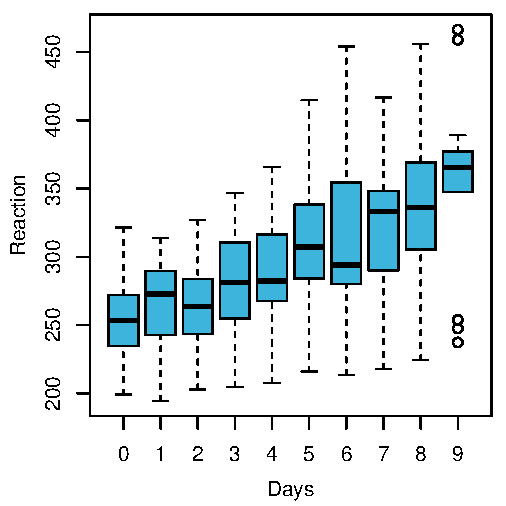
\includegraphics[scale=.8]{fig/sleep_box}
    \end{column}
    \begin{column}{.55\textwidth}
\begin{lstlisting}
boxplot(Reaction ~ Days, sleepstudy)
\end{lstlisting}
    \end{column}
  \end{columns}
\end{frame}

\begin{frame}[fragile]{Visualization of individual data}
  \begin{columns}
    \begin{column}{.53\textwidth}
      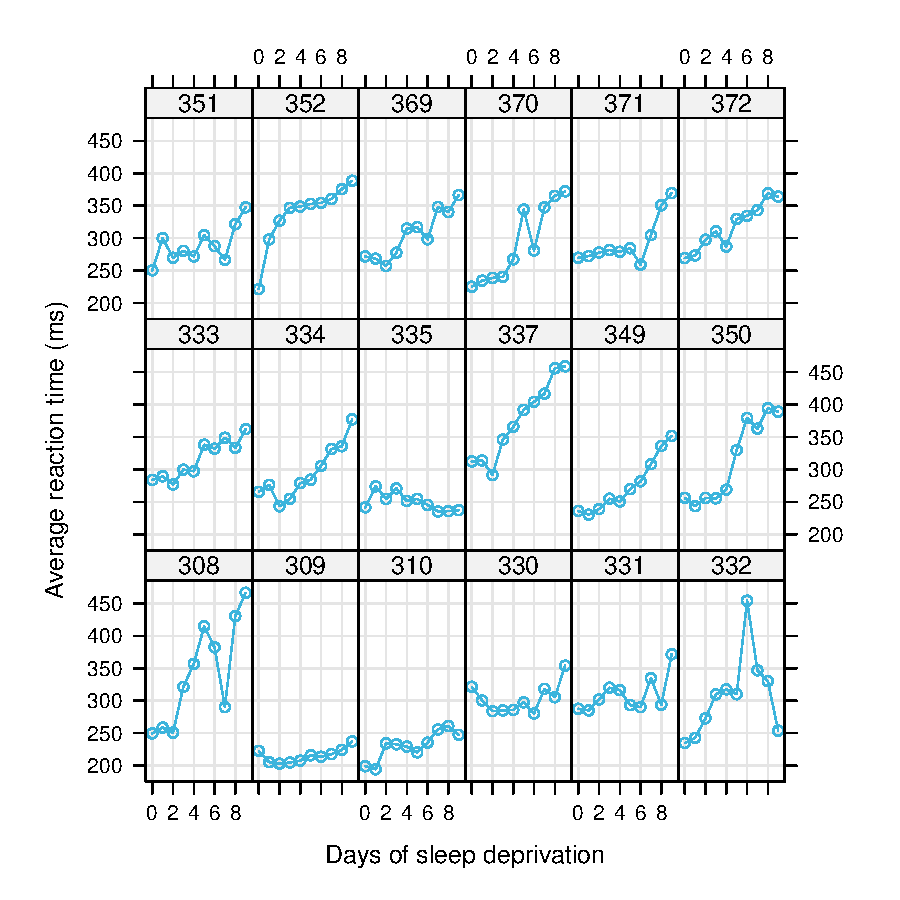
\includegraphics[scale=.5]{fig/sleep_subjects}
    \end{column}
    \begin{column}{.55\textwidth}
\begin{lstlisting}
library(lattice)

xyplot(Reaction ~ Days | Subject,
  data = sleepstudy,
  type = c("g", "b"),
  xlab = "Days of sleep deprivation",
  ylab = "Average reaction time (ms)",
  aspect = "xy")
\end{lstlisting}
    \end{column}
  \end{columns}
\end{frame}

\begin{frame}{Random intercept model}
  \begin{columns}
    \begin{column}{.5\textwidth}
  \begin{itemize}
\item The random intercept model adds a random intercept for each subject
\[
  y_{ij} = \beta_0 + \beta_1\,Days_{ij} + \upsilon_{0i} + \varepsilon_i
\]
with $\upsilon_{0i} \overset{iid}{\sim} N(0, \sigma^2_{\upsilon})$,
      $\varepsilon_{ij} \overset{iid}{\sim} N(0, \sigma^2)$
    \item The slope is identical for each subject (and the population)
  \end{itemize}
      \vspace{2.2cm}
    \end{column}
    \begin{column}{.5\textwidth}
      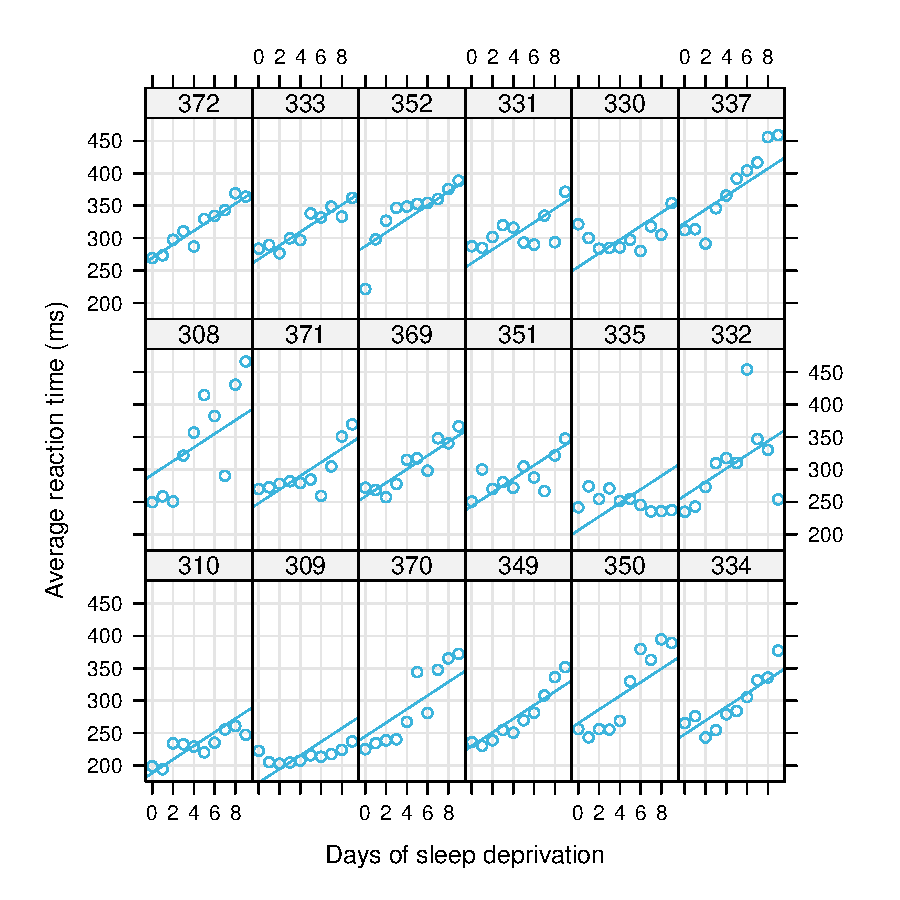
\includegraphics[scale=.5]{fig/sleep_random_intercept}
    \end{column}
  \end{columns}
\end{frame}

% \begin{align*}
% \text{(Level 1)}  \quad y_{ij} &= b_{0i} + b_{1i}\,Days_{ij} + \varepsilon_{ij}\\
% \text{(Level 2)}  \quad b_{0i} &= \beta_0 + \upsilon_{0i}\\
%                   \quad b_{1i} &= \beta_1\\
% \text{(2) in (1)} \quad y_{ij} &= \beta_0 + \beta_1\,Days_{ij} +
%                                   \upsilon_{0i} + \varepsilon_{ij}
% \end{align*}
% \vfill
% with $\upsilon_{0i} \sim N(0, \sigma^2_{\upsilon})$ i.i.d.,
% $\varepsilon_{ij} \sim N(0, \sigma^2)$ i.i.d., $\upsilon_{0i}$ and
% $\varepsilon_{ij}$ i.i.d.\\[2ex]
% \vfill

% \begin{frame}[fragile]{Random intercept model}
% \begin{lstlisting}
% lme0 <- lmer(Reaction ~ Days + (1 | Subject), sleepstudy)
% summary(lme0)
% 
% # model matrices
% X <- model.matrix(~ Days, sleepstudy)
% Z <- model.matrix(~ 0 + Subject, sleepstudy)
% 
% # coefficients
% coef(lme0)
% fixef(lme0)
% ranef(lme0)
% \end{lstlisting}
% \end{frame}

\begin{frame}[fragile]{Random slope model}
  \begin{columns}
    \begin{column}{.5\textwidth}
  \begin{itemize}
\item The random slope model adds a random intercept and a random slope for each
  subject
\[
  y_{ij} = \beta_0 + \beta_1\,Days_{ij} + \upsilon_{0i} +
      \upsilon_{1i}\,Days_{ij} + \varepsilon_{ij}
\]
with
\begin{align*}
  \begin{pmatrix} \upsilon_{0i}\\ \upsilon_{1i} \end{pmatrix} &\overset{iid}{\sim}
    N \left(\begin{pmatrix} 0\\ 0 \end{pmatrix}, \, \gmat{\Sigma}_\upsilon =
      \begin{pmatrix}
        \sigma^2_{\upsilon_0} & \sigma_{\upsilon_0 \upsilon_1} \\
        \sigma_{\upsilon_0 \upsilon_1} & \sigma^2_{\upsilon_1} \\
      \end{pmatrix} \right)
    \\
  \varepsilon_{ij} & \overset{iid}{\sim} N(0, \sigma_{\varepsilon}^2)
\end{align*}
      \vspace{-.5cm}
    \item Individual slopes for each subject
  \end{itemize}
    \end{column}
    \begin{column}{.5\textwidth}
      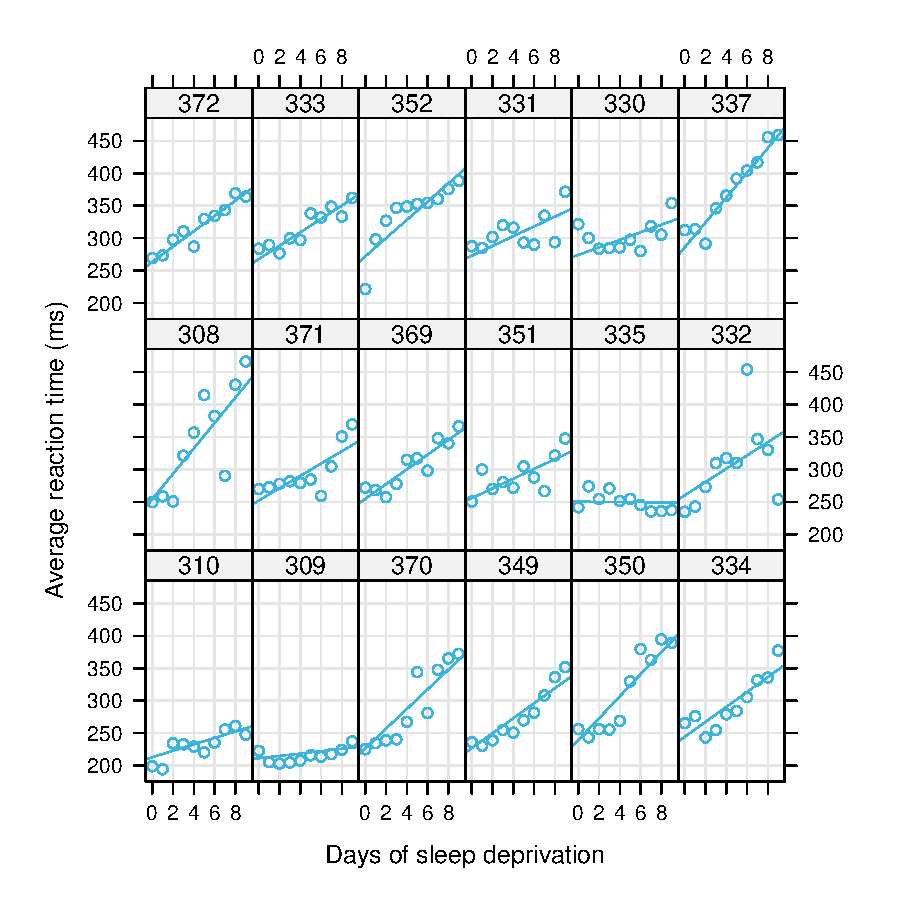
\includegraphics[scale=.5]{fig/sleep_random_slope}
    \end{column}
  \end{columns}
\end{frame}

% \begin{frame}[fragile]{Random slope model}
% \begin{lstlisting}
% lme1 <- lmer(Reaction ~ Days + (Days | Subject), sleepstudy)
% summary(lme1)
% 
% # model matrices
% X <- model.matrix(~ Days, sleepstudy)
% Z <- model.matrix(~ 0 + Subject + Subject:Days, sleepstudy)
% 
% # coefficients
% coef(lme1)
% fixef(lme1)
% ranef(lme1)
% \end{lstlisting}
% \end{frame}

% \begin{frame}[fragile]{Model with uncorrelated random effects}
%   \begin{itemize}
%     \item We will now consider a model without correlated random effects
%   \[
%     y_{ij} = \beta_0 + \beta_1 Days_{ij} + \upsilon_{0i} + \upsilon_{1i} Days_{ij} +
%     \varepsilon_{ij}
%   \]
% with
%       \[
%   \gvect{\upsilon}  \overset{iid}{\sim} N\left(\gvect{0}, \gmat{\Sigma}_{\upsilon} = 
%     \begin{pmatrix}
%       \sigma^2_{\upsilon_0} & 0 \\
%       0 & \sigma^2_{\upsilon_1} \\
%     \end{pmatrix}\right) ~~~\text{and}~~~
%   \varepsilon_{ij}  \overset{iid}{\sim} N(0, \sigma_{\varepsilon}^2)
% \]
%   \end{itemize}
%   \begin{lstlisting}
% lme2 <- lmer(Reaction ~ Days + (Days || Subject), sleepstudy)
% summary(lme2)
% 
% # likelihood-ratio test
% anova(lme1, lme2)
% # confidence intervals
% confint(lme2)
%   \end{lstlisting}
% \end{frame}

% \begin{frame}{Confidence intervals and interpretation}
%   \begin{itemize}
%     \item The results indicate that the extra parameter
%       $\sigma_{\upsilon_0\upsilon_1}$ does not produce a significantly
%       better fit
%     \item Results show that we have a significant effect for days with an
%   average increase in reaction time of 10.47\,ms for each day of sleep
%   deprivation
%     \item We get an estimate of $\sigma_{\upsilon_0} = 24.17$ for the
%       standard deviation of reaction time for subjects and a standard
%       deviation of $\sigma_{\upsilon_1} = 5.80$ for the dependence of
%       reaction time on days of sleep deprivation
%   \end{itemize}
% \end{frame}
% 
% \begin{frame}[fragile]{Examining random effects and predictions}
%       \begin{lstlisting}
% coef(lme2)
% fixef(lme2)
% ranef(lme2)
% 
% # correlational structure for intercepts and slopes
% dotplot(ranef(lme2, condVar = TRUE),
%         scales = list(x = list(relation = "free")))[[1]]
% 
% # predictions for all subjects
% predict(lme2)
%       \end{lstlisting}
% \end{frame}

% \begin{frame}[fragile]{Examining random effects and predictions}
%   \begin{center}
%     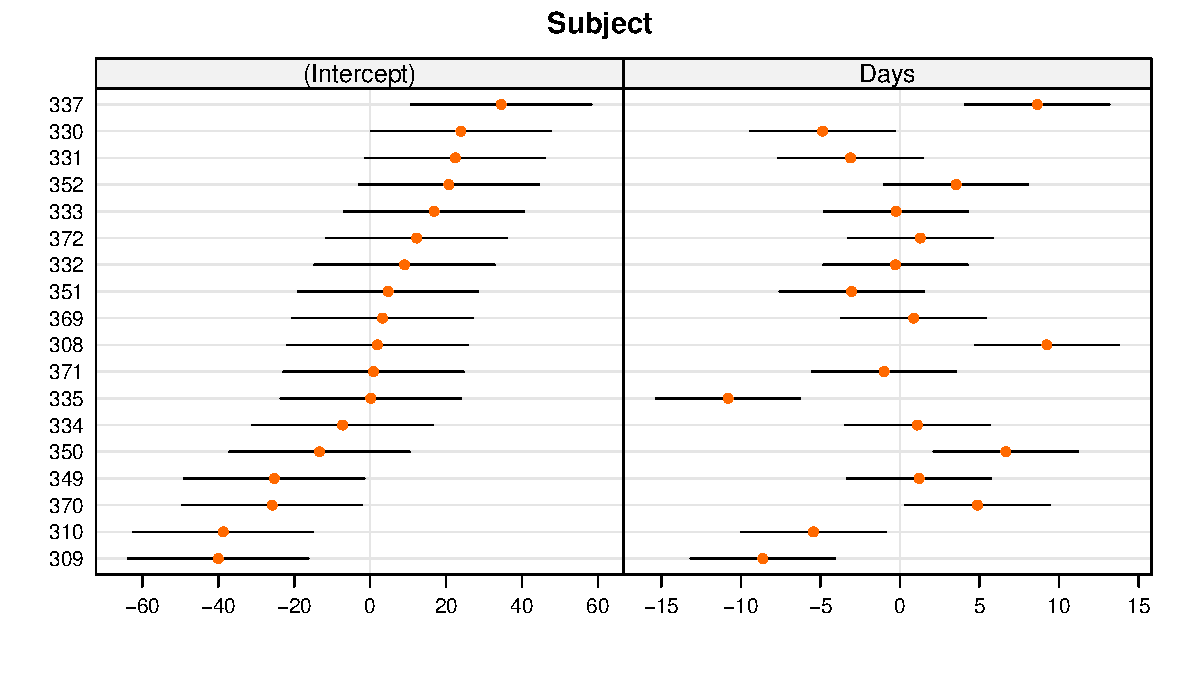
\includegraphics[scale=.6]{fig/sleep_caterpillar}
%   \end{center}
% \end{frame}

\begin{frame}{Partial pooling}
  \begin{columns}
    \begin{column}{.5\textwidth}
      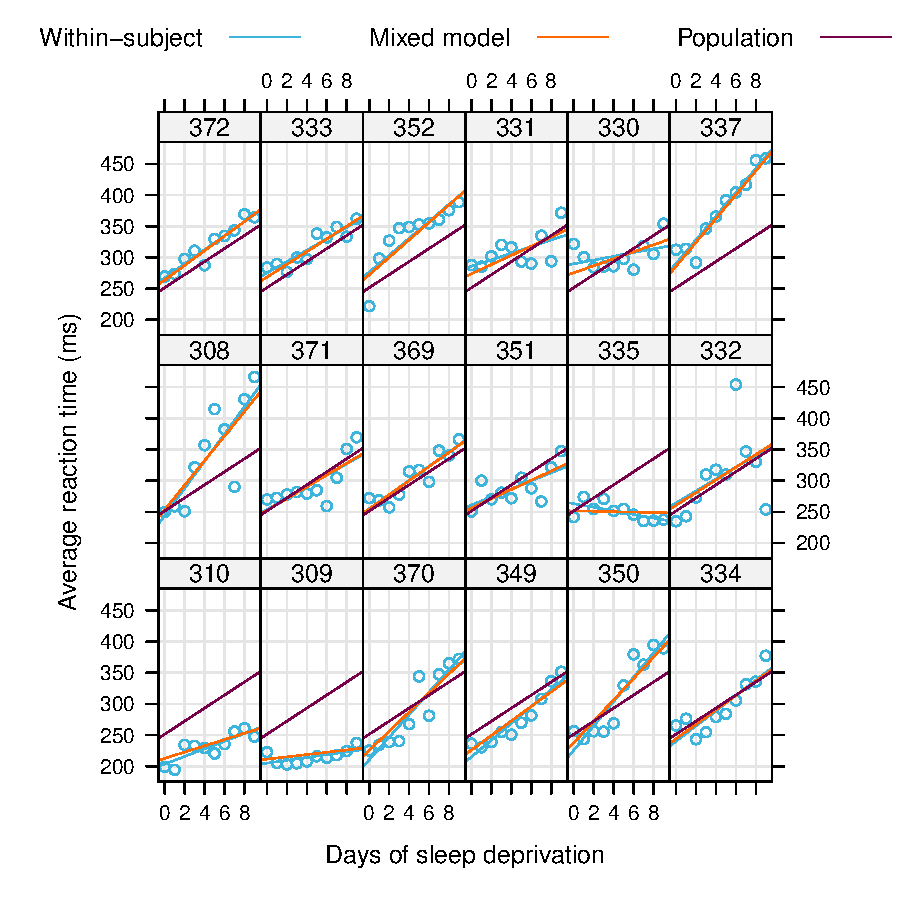
\includegraphics[scale=.5]{fig/sleep_shrinkfit}
    \end{column}
    \begin{column}{.5\textwidth}
      \begin{itemize}
        \item Within-subject regression line shows regression line fitted to
          data for each individual
        \item Population regression line shows fixed effects for mixed-effects
          model
        \item Mixed model regression line shows individual regression lines as
          predicted by mixed-effects models
      \end{itemize}
    \end{column}
  \end{columns}
\end{frame}

% \begin{frame}{Shrinkage}
%   \begin{columns}
%     \begin{column}{.5\textwidth}
%   \begin{itemize}
%     \item When per-subject slopes and intercepts calculated from a
%       mixed-effects model are compared to estimated slopes and intercepts
%       within subjects, estimates from mixed-effects model are
%       closer to the population estimates (the fixed effects)
%     \item This pattern is sometimes described as {\it shrinkage} of
%       coefficients toward the population values
%     \item The more within-subject variance, the stronger parameters {\it shrink}
%       towards the population parameters
%     % \item In a mixed-effects model, we assume that the levels of a grouping
%     %   factor are a selection from a population and, as a result, can be
%     %   expected to share characteristics to some degree
%   \end{itemize}
%     \end{column}
%     \begin{column}{.5\textwidth}
%     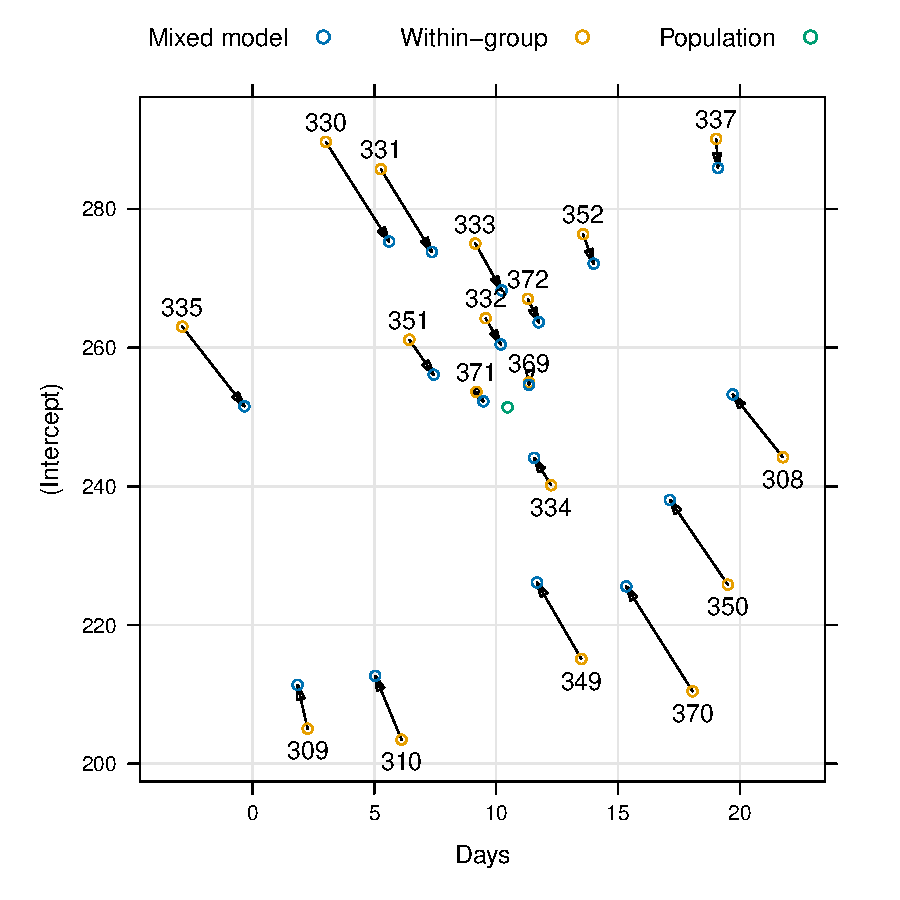
\includegraphics[scale=.48]{fig/sleep_shrinkage}
%     \end{column}
%   \end{columns}
% \end{frame}

% \begin{frame}[fragile]{Assumptions}
%   \begin{columns}
%     \begin{column}{.5\textwidth}
%       \begin{itemize}
%         \item Assumptions can be checked visually
%         \item Normality assumption
%           \begin{lstlisting}
% qqmath(lme2,
%      col = sleepstudy$Subject,
%      pch = sleepstudy$Days)
%           \end{lstlisting}
%         \item Independence assumption
%           \begin{lstlisting}
% plot(lme2,
%      col = sleepstudy$Subject,
%      pch = sleepstudy$Days)
%           \end{lstlisting}
%       \end{itemize}
%       {\tiny \url{https://bbolker.github.io/morelia_2018/notes/mixedlab.html}}
%     \end{column}
%     \begin{column}{.5\textwidth}
%       \includegraphics[scale=.5]{fig/assump_qqplot_slope.pdf}
%     \end{column}
%   \end{columns}
% \end{frame}
% 
% \begin{frame}{Assumptions}
%   \begin{columns}
%     \begin{column}{.5\textwidth}
%       \includegraphics[scale=.5]{fig/assump_resid_slope.pdf}
%     \end{column}
%     \begin{column}{.5\textwidth}
%       \includegraphics[scale=.5]{fig/assump_resid_intercept.pdf}
%     \end{column}
%   \end{columns}
% \end{frame}

% \section{Parameter estimation}
% 
% \begin{frame}{Maximum Likelihood Estimation}
%   \begin{itemize}
%     \item The maximum likelihood principle was introduced by
%       R.\,A.\ Fisher
%       \begin{itemize}
%       \item It can be used for almost all estimation problems, also complex
%         ones
%       \item The resulting estimation functions have many desirable
%         properties
%       \end{itemize}
%     \item Obtaining the MLE $\hat{\vartheta}$ takes the
%       following steps\\[1ex]
%     \begin{enumerate}
%       \item Generate the log-likelihood
%       \[
%         \log L(\vartheta)
%       \]
%       \vspace{-3ex}
%       \item Take the derivative of the log-likelihood with respect to
%         parameter $\vartheta$
%       \[
%         (\log L)' (\vartheta) = \frac{d \log L(\vartheta)}{d \vartheta}
%       \]
%       \vspace{-3ex}
%       \item Set the derivative equal to 0
%       \[
%         (\log L)' (\hat{\vartheta}) = 0
%       \]
%       \vspace{-3ex}
%       \item Solve the resulting equation for the estimator $\hat{\vartheta}$
%     \end{enumerate}
%   \end{itemize}
% \end{frame}
% 
% \begin{frame}{Restricted Maximum Likelihood Estimation}
%   \begin{itemize}
%     \item The restricted maximum likelihood (REML) approach is a form of Maximum
%       Likelihood Estimation
%     \item In particular, REML is used as a method for fitting linear
%       mixed-effects models
%     \item In contrast to traditional Maximum Likelihood Estimation, REML can
%       produce unbiased estimates of variance and covariance parameters
%     \item MLE and REML do not outmatch each other, both can be used
%     \item REML is the default in \texttt{lme4}, but if we want to conduct
%       likelihood ratio tests, only MLE estimates are valid
%   \end{itemize}
% \end{frame}

\section{Crossed random effects}

\begin{frame}{Crossed random effects}
  \begin{itemize}
    % \item Crossed random effects are fitted for cross-classified data (each
    %   level of one factor is crossed with each level of the other factor)
    \item In many experiments in psychology the reaction of each subject ($j =
      1, \dots, N$) to a complete set of stimuli or items ($k = 1, \dots, K$) is
      measured
  \[
    y_{ijk} = \beta_0 + \beta_ix_{i} + \upsilon_{0j} + \eta_{0k} + \varepsilon_{ijk}
  \]
  with $\varepsilon_{ijk} \overset{iid}{\sim} N(0,\sigma^2)$, 
  $\upsilon_{0j} \overset{iid}{\sim} N(0,\sigma^2_{\upsilon})$, and 
  $\eta_{0k} \overset{iid}{\sim} N(0,\sigma^2_{\eta})$

    \item Data are completely crossed: all subjects are presented with all items
  \end{itemize}
  \footnotesize
  \begin{center}
  \begin{tabular}{lcccccc}
    & & \multicolumn{5}{c}{Subject}\\
    \cline{3-7}
     & & 1 & 2 & 3 & \dots & 20 \\
    \hline
      & 1 & $1$ & $1$ & $1$ & \dots & $1$ \\
      & 2 & $1$ & $1$ & $1$ & \dots & $1$ \\
Item  & 3 & $1$ & $1$ & $1$ & \dots & $1$ \\
      & \vdots & \vdots & \vdots & \vdots & \vdots & \vdots\\
      & 10 & $1$ & $1$ & $1$ & \dots & $1$ \\
      \hline
  \end{tabular}
  \end{center}
\end{frame}

% \begin{frame}[fragile]{Crossed random effects}
%   \vspace{-.6cm}
%   \begin{columns}
%     \begin{column}[t]{4.5cm}
%   \begin{lstlisting}
% > head(dat, 12)
%    id  cond   item  av
% 1   1 cond1 item01 105
% 2   1 cond1 item02 116
% 3   1 cond1 item03 104
% 4   1 cond1 item04  81
% 5   1 cond1 item05  99
% 6   1 cond1 item06 109
% 7   1 cond1 item07 100
% 8   1 cond1 item08 103
% 9   1 cond1 item09  89
% 10  1 cond1 item10  94
% 11  2 cond1 item01 107
% 12  2 cond1 item02 100
%   \end{lstlisting}
%     \end{column}
% 
%     \begin{column}[t]{7cm}
%   \begin{lstlisting}
% > xtabs( ~ item + id, dat)
%         id
% item     1 2 3 4 5 6 7 8 9 ... 20
%   item01 1 1 1 1 1 1 1 1 1 ...  1
%   item02 1 1 1 1 1 1 1 1 1 ...  1
%   item03 1 1 1 1 1 1 1 1 1 ...  1
%   item04 1 1 1 1 1 1 1 1 1 ...  1
%   item05 1 1 1 1 1 1 1 1 1 ...  1
%   item06 1 1 1 1 1 1 1 1 1 ...  1
%   item07 1 1 1 1 1 1 1 1 1 ...  1
%   item08 1 1 1 1 1 1 1 1 1 ...  1
%   item09 1 1 1 1 1 1 1 1 1 ...  1
%   item10 1 1 1 1 1 1 1 1 1 ...  1
%   \end{lstlisting}
%     \end{column}
%   \end{columns}
% \end{frame}

\begin{frame}{Lexical decision task \citep{Baayen2008}}
  \begin{itemize}
    \item Assume an example data set with three participants s1, s2 and s3
      who each saw three items w1, w2, w3 in a priming lexical decision
      task under both short and long stimulus onset asynchrony (SOA) conditions
    \item The data are generated by the following model with random intercepts
      for subject and item, and random slopes for subject
  \[
    y_{ijk} = \beta_0 + \beta_1 SOA_k + \eta_{0j} + \upsilon_{0i} +
      \upsilon_{1i} SOA_k + \varepsilon_{ijk} 
  \]
\small
with $\gvect{\upsilon} \sim N\left(\gvect{0}, \gmat{\Sigma}_{\upsilon} = 
    \begin{pmatrix}
      \sigma^2_{\upsilon_0} & \sigma_{\upsilon_0\upsilon_1} \\
      \sigma_{\upsilon_0\upsilon_1} & \sigma^2_{\upsilon_1} \\
    \end{pmatrix}\right)$,
      $\eta_{0j} \sim N(0, \sigma_{\eta}^2)$, $\varepsilon_{ijk} \sim N(0,
  \sigma_{\varepsilon}^2)$, all i.i.d. 
  \end{itemize}
\end{frame}

\begin{frame}{Structure of the data set}
  \begin{columns}
    \begin{column}{.4\textwidth}
      \centering
  \scriptsize
  \begin{tabular}{llll}
    \hline
    Subj & Item & SOA & RT  \\
    \hline
    s1 & w1 & Long  & 466 \\
    s1 & w2 & Long  & 520 \\
    s1 & w3 & Long  & 502 \\
    s1 & w1 & Short & 475 \\
    s1 & w2 & Short & 494 \\
    s1 & w3 & Short & 490 \\
    s2 & w1 & Long  & 516 \\
    s2 & w2 & Long  & 566 \\
    s2 & w3 & Long  & 577 \\
    s2 & w1 & Short & 491 \\
    s2 & w2 & Short & 544 \\
    s2 & w3 & Short & 526 \\
    s3 & w1 & Long  & 484 \\
    s3 & w2 & Long  & 529 \\
    s3 & w3 & Long  & 539 \\
    s3 & w1 & Short & 470 \\
    s3 & w2 & Short & 511 \\
    s3 & w3 & Short & 528 \\
    \hline
  \end{tabular}
    \end{column}
    \begin{column}{.6\textwidth}
      \begin{itemize}
        \item When we collect data, we might get a data set like this
        \item We fit a model to the data to separate the structural and the
          stochastical parts
      \end{itemize}
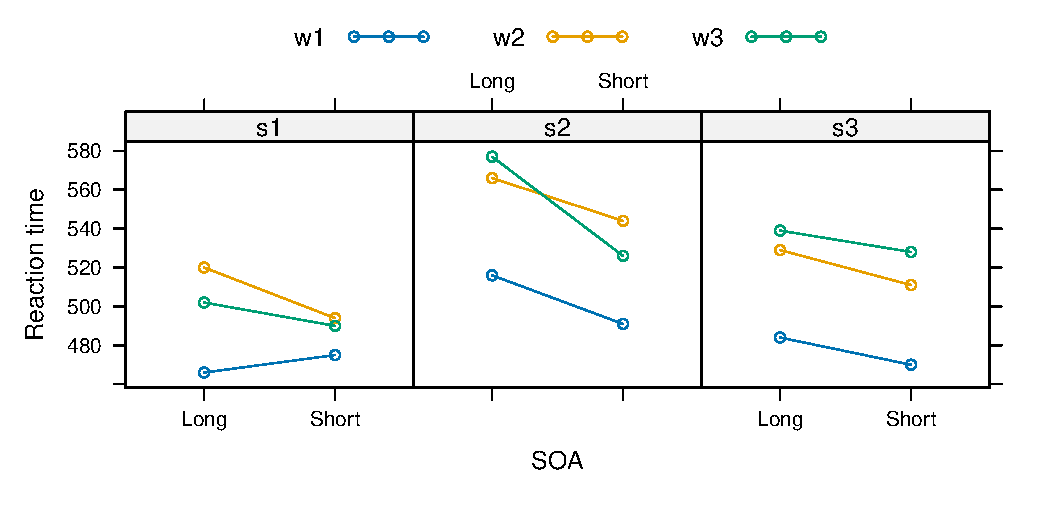
\includegraphics[scale=.5]{fig/baayen_ex}
    \end{column}
  \end{columns}
\end{frame}

\begin{frame}{Aggregated data}
  \begin{center}
    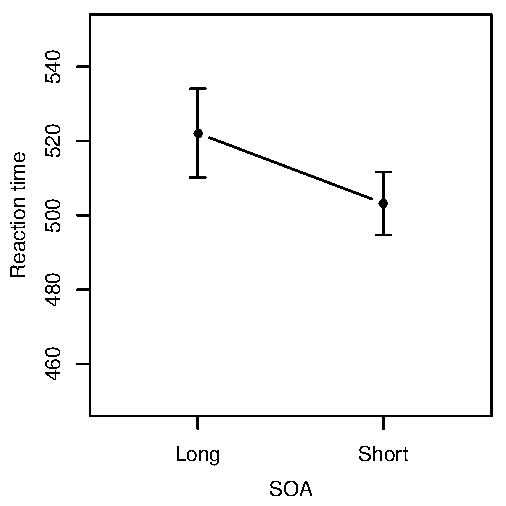
\includegraphics[scale=.8]{fig/baayen_ex_agg}
  \end{center}
\end{frame}

\begin{frame}{Structure of the data set}
  \vspace{.2cm}
  \scriptsize
  \centering
  \begin{tabular}{llllcrrrcr}
    \hline
    Subj & Item & SOA & RT & Fixed &&  Random &&& Res \\
    \cline{5-6}
    \cline{7-10}
    & & & & Int & SOA & ItemInt & SubInt & SubSOA & \\
    \hline
    s1 & w1 & Long  & 466 & 522.2 & 0     & $-$28.3 & $-$26.2 & 0       & $-$2.0 \\
    s1 & w2 & Long  & 520 & 522.2 & 0     & 14.2    & $-$26.2 & 0       & 9.8 \\
    s1 & w3 & Long  & 502 & 522.2 & 0     & 14.1    & $-$26.2 & 0       & $-$8.2 \\
    s1 & w1 & Short & 475 & 522.2 & $-$19 & $-$28.3 & $-$26.2 & 11      & 15.4 \\
    s1 & w2 & Short & 494 & 522.2 & $-$19 & 14.2    & $-$26.2 & 11      & $-$8.4 \\
    s1 & w3 & Short & 490 & 522.2 & $-$19 & 14.1    & $-$26.2 & 11      & $-$11.9 \\
    s2 & w1 & Long  & 516 & 522.2 & 0     & $-$28.3 & 29.7    & 0       & $-$7.4 \\
    s2 & w2 & Long  & 566 & 522.2 & 0     & 14.2    & 29.7    & 0       & 0.1 \\
    s2 & w3 & Long  & 577 & 522.2 & 0     & 14.1    & 29.7    & 0       & 11.5 \\
    s2 & w1 & Short & 491 & 522.2 & $-$19 & $-$28.3 & 29.7    & $-$12.5 & $-$1.5 \\
    s2 & w2 & Short & 544 & 522.2 & $-$19 & 14.2    & 29.7    & $-$12.5 & 8.9 \\
    s2 & w3 & Short & 526 & 522.2 & $-$19 & 14.1    & 29.7    & $-$12.5 & $-$8.2 \\
    s3 & w1 & Long  & 484 & 522.2 & 0     & $-$28.3 & $-$3.5  & 0       & $-$6.3 \\
    s3 & w2 & Long  & 529 & 522.2 & 0     & 14.2    & $-$3.5  & 0       & $-$3.5 \\
    s3 & w3 & Long  & 539 & 522.2 & 0     & 14.1    & $-$3.5  & 0       & 6.0 \\
    s3 & w1 & Short & 470 & 522.2 & $-$19 & $-$28.3 & $-$3.5  & 1.5     & $-$2.9 \\
    s3 & w2 & Short & 511 & 522.2 & $-$19 & 14.2    & $-$3.5  & 1.5     & $-$4.6 \\
    s3 & w3 & Short & 528 & 522.2 & $-$19 & 14.1    & $-$3.5  & 1.5     & 13.2 \\
    \hline
    &&&&&& $\sigma^2_{\eta_0}$ & $\sigma^2_{\upsilon_0}$ &
    $\sigma^2_{\upsilon_1}$ & $\sigma^2_{\varepsilon}$\\ 
    &&&&&&  & \multicolumn{2}{c}{$\sigma_{\upsilon_0\upsilon_1}$} & 
  \end{tabular}
\end{frame}

\begin{frame}{True values}
  \begin{itemize}
    \item We assume the following true parameters for a data simulation
    \vspace{.2cm}
  \begin{center}
  \begin{tabular}{lrr}
    \hline
    Parameter && Model \\
    \hline
    $\beta_0$                     && 522.22\\
    $\beta_1$                     && $-$19.00\\
    $\sigma_{\eta}$               && 21.00\\
    $\sigma_{\upsilon_0}$         && 24.00\\
    $\sigma_{\upsilon_1}$         && 7.00\\
    $\rho_{\upsilon_0\upsilon_1}$ && $-$0.70\\
    $\sigma_{\varepsilon}$        && 9.00\\
    \hline
  \end{tabular}
  \end{center}
     \[
       y_{ijk} = \beta_0 + \beta_1 SOA_k + \eta_{0j} + \upsilon_{0i} +
       \upsilon_{1i} SOA + \varepsilon_{ijk} 
  \]
\small
with $\gvect{\upsilon} \sim N\left(\gvect{0}, \gmat{\Sigma}_{\upsilon} = 
    \begin{pmatrix}
      \sigma^2_{\upsilon_0} & \sigma_{\upsilon_0\upsilon_1} \\
      \sigma_{\upsilon_0\upsilon_1} & \sigma^2_{\upsilon_1} \\
    \end{pmatrix}\right)$,
  $\eta_{0j} \sim N(0, \sigma_{\eta}^2)$, $\varepsilon_{ijk} \sim N(0,
  \sigma_{\varepsilon}^2)$ 
  \end{itemize}
\end{frame}

% \begin{frame}[fragile]{Fixed effects}
%   \begin{lstlisting}
% datsim <- expand.grid(subject = factor(c("s1", "s2", "s3")),
%                       item    = factor(c("w1", "w2", "w3")),
%                       soa     = factor(c("long", "short"))) |>
%   sort_by( ~ subject)
% 
% # model matrix in dummy coding
% model.matrix(~ soa, datsim)
% 
% beta0 <- 522.11
% beta1 <- -18.89
% b0 <- rep(beta0, 18)
% b1 <- rep(rep(c(0, beta1), each = 3), 3)
% cbind(b0, b1)
%   \end{lstlisting}
% \end{frame}

% \begin{frame}[fragile]{Random effects}
%   \begin{lstlisting}
% sw  <- 21.1
% sy0 <- 23.89; sy1 <- 9; ry <- -1
% se  <- 9.9
% 
% w  <- rep(rnorm(3, mean = 0, sd = sw), 6)
% e  <- rnorm(18, mean = 0, sd = se)
% # draw from bivariate normal distribution
% sig <- matrix(c(sy0^2, ry * sy0 * sy1, ry * sy0 * sy1, sy1^2), 2, 2)
% y01 <- mvtnorm::rmvnorm(3, mean = c(0, 0), sigma = sig)
% y0 <- rep(y01[,1], each = 6)
% y1 <- rep(c(0, y01[1,2],
%             0, y01[2,2],
%             0, y01[3,2]), each = 3)
% cbind(w, y0, y1, e)
%   \end{lstlisting}
% \end{frame}

% \begin{frame}[fragile]{Simulate data}
%   \begin{lstlisting}
% datsim$rt <- b0 + b1 + w + y0 + y1 + e
% 
% # fit model
% library(lme4)
% 
% lme1 <- lmer(rt ~ soa + (1 | item) + (soa | subject), data = datsim)
% summary(lme1)
% confint(lme1)
% 
% # btw
% ?pvalues
% ?convergence
%   \end{lstlisting}
% \end{frame}

% \begin{frame}{Comparison of sample and model estimates}
%   For this example, we are able to compare the ``true'' values to the
%   parameter estimates
%   \begin{center}
%   \begin{tabular}{lrrrr}
%     \hline
%     Parameter && Sample && Model \\
%     \hline
%     $\hat\beta_0$ && 522.2 && 522.11\\
%     $\hat\beta_1$ && $-$19.00 && $-$18.89\\
%     $\hat\sigma_{\eta}$ && 20.59 && 21.10\\
%     $\hat\sigma_{\upsilon_0}$ && 23.62 && 23.89\\
%     $\hat\sigma_{\upsilon_1}$ && 9.76 && 9.00\\
%     $\hat\rho_{\upsilon_0\upsilon_1}$ && $-$0.71 && $-$1.00\\
%     $\hat\sigma_{\varepsilon}$ && 8.55 && 9.90\\
%     \hline
%   \end{tabular}
%   \end{center}
%      \[
%        y_{ijk} = \beta_0 + \beta_1 SOA_k + \eta_{0j} + \upsilon_{0i} +
%        \upsilon_{1i} SOA_k + \varepsilon_{ijk} 
%   \]
% \small
% with $\gvect{\upsilon} \sim N\left(\gvect{0}, \gmat{\Sigma}_{\upsilon} = 
%     \begin{pmatrix}
%       \sigma^2_{\upsilon_0} & \sigma_{\upsilon_0\upsilon_1} \\
%       \sigma_{\upsilon_0\upsilon_1} & \sigma^2_{\upsilon_1} \\
%     \end{pmatrix}\right)$,
%   $\eta_{0j} \sim N(0, \sigma_{\eta}^2)$, $\varepsilon_{ijk} \sim N(0,
%   \sigma_{\varepsilon}^2)$ 
% \end{frame}


% \begin{frame}{Linear mixed-effects model}
%   \begin{itemize}
%     \item The linear mixed-effects model has the general form
% \[
%   \vect{y}_i = \mat{X}_i \, \gvect{\beta} + \mat{Z}_i \, \gvect{\upsilon}_i +
%                \gvect{\varepsilon}_i
% \]
% with fixed effects $\gvect{\beta}$, random effects
% $\gvect{\upsilon}_i$, and the design matrices $\mat{X}_i$ and $\mat{Z}_i$
%   and the assumptions
% \[
%   \gvect{\upsilon}_i \sim N(\vect{0}, \, \gmat{\Sigma}_\upsilon)
%     \text{ i.i.d.}, \qquad
%   \gvect{\varepsilon}_i \sim N(\vect{0}, \, \sigma^2 \mat{I}_{n_i})
%     \text{ i.i.d.}
% \]
%   \end{itemize}
% \end{frame}

% \begin{frame}[shrink=10]{Linear mixed-effects model}
% \vspace{2cm}
% \begin{equation*}
%   \begin{pmatrix}
%     y_1 \\
%     y_2 \\
%     y_3 \\
%     \vdots \\
%     y_N
%   \end{pmatrix} = 
%   \begin{pmatrix}
%     1 & x_{11} & x_{12} & \dots & x_{1p} \\
%     1 & x_{21} & x_{22} & \dots & x_{2p} \\
%     1 & x_{31} & x_{32} & \dots & x_{3p} \\
%     \vdots & \vdots & \vdots & \vdots & \vdots \\
%     1 & x_{N1} & x_{N2} & \dots & x_{Np} \\
%   \end{pmatrix} \cdot
%   \begin{pmatrix}
%     \beta_0 \\
%     \beta_1 \\
%     \vdots \\
%     \beta_p
%   \end{pmatrix} +
%   \begin{pmatrix}
%     z_{10} & z_{11} & \dots & z_{1q} & \dots \\
%     z_{20} & z_{21} & \dots & z_{2q} & \dots \\
%     z_{30} & z_{31} & \dots & z_{3q} & \dots \\
%     \vdots & \vdots & \vdots & \vdots & \vdots \\
%     z_{N0} & z_{N1} & \dots & z_{Nq} & \dots \\
%   \end{pmatrix} \cdot
%   \begin{pmatrix}
%     \upsilon_{10} \\
%     \vdots \\
%     \upsilon_{1q}\\
%     \upsilon_{20} \\
%     \vdots \\
%     \upsilon_{Nq}
%   \end{pmatrix} + 
%   \begin{pmatrix}
%     \varepsilon_1 \\
%     \varepsilon_2 \\
%     \varepsilon_3 \\
%     \vdots \\
%     \varepsilon_N
%   \end{pmatrix}
% \end{equation*}
% \end{frame}

\begin{frame}{Matrix notation}
For this simple example the model looks like this in matrix notation
\scriptsize
\begin{equation*}
  \begin{pmatrix}
    y_{111} \\
    y_{121} \\
    y_{131} \\
    y_{112} \\
    y_{122} \\
    y_{132} \\
    y_{211} \\
    y_{221} \\
    y_{231} \\
    y_{212} \\
    y_{222} \\
    y_{232} \\
    y_{311} \\
    y_{321} \\
    y_{331} \\
    y_{312} \\
    y_{322} \\
    y_{332}
  \end{pmatrix} =
  \begin{pmatrix}
    1 & 0 \\
    1 & 0 \\
    1 & 0 \\
    1 & 1 \\
    1 & 1 \\
    1 & 1 \\
    1 & 0 \\
    1 & 0 \\
    1 & 0 \\
    1 & 1 \\
    1 & 1 \\
    1 & 1 \\
    1 & 0 \\
    1 & 0 \\
    1 & 0 \\
    1 & 1 \\
    1 & 1 \\
    1 & 1
  \end{pmatrix} \cdot
  \begin{pmatrix}
    \beta_0 \\
    \beta_1
  \end{pmatrix} +
  \begin{pmatrix}
    1 & 0 & 0 & 1 & 0 & 0 & 0 & 0 & 0 \\
    0 & 1 & 0 & 1 & 0 & 0 & 0 & 0 & 0 \\
    0 & 0 & 1 & 1 & 0 & 0 & 0 & 0 & 0 \\
    1 & 0 & 0 & 1 & 0 & 0 & 1 & 0 & 0 \\
    0 & 1 & 0 & 1 & 0 & 0 & 1 & 0 & 0 \\
    0 & 0 & 1 & 1 & 0 & 0 & 1 & 0 & 0 \\
    1 & 0 & 0 & 0 & 1 & 0 & 0 & 0 & 0 \\
    0 & 1 & 0 & 0 & 1 & 0 & 0 & 0 & 0 \\
    0 & 0 & 1 & 0 & 1 & 0 & 0 & 0 & 0 \\
    1 & 0 & 0 & 0 & 1 & 0 & 0 & 1 & 0 \\
    0 & 1 & 0 & 0 & 1 & 0 & 0 & 1 & 0 \\
    0 & 0 & 1 & 0 & 1 & 0 & 0 & 1 & 0 \\
    1 & 0 & 0 & 0 & 0 & 1 & 0 & 0 & 0 \\
    0 & 1 & 0 & 0 & 0 & 1 & 0 & 0 & 0 \\
    0 & 0 & 1 & 0 & 0 & 1 & 0 & 0 & 0 \\
    1 & 0 & 0 & 0 & 0 & 1 & 0 & 0 & 1 \\
    0 & 1 & 0 & 0 & 0 & 1 & 0 & 0 & 1 \\
    0 & 0 & 1 & 0 & 0 & 1 & 0 & 0 & 1
  \end{pmatrix} \cdot
  \begin{pmatrix}
    \eta_{01} \\
    \eta_{02} \\
    \eta_{03} \\
    \upsilon_{01}\\
    \upsilon_{02} \\
    \upsilon_{03} \\
    \upsilon_{11}\\
    \upsilon_{12} \\
    \upsilon_{13}
  \end{pmatrix} +
  \begin{pmatrix}
    \varepsilon_{111} \\
    \varepsilon_{121} \\
    \varepsilon_{131} \\
    \varepsilon_{112} \\
    \varepsilon_{122} \\
    \varepsilon_{132} \\
    \varepsilon_{211} \\
    \varepsilon_{221} \\
    \varepsilon_{231} \\
    \varepsilon_{212} \\
    \varepsilon_{222} \\
    \varepsilon_{232} \\
    \varepsilon_{311} \\
    \varepsilon_{321} \\
    \varepsilon_{331} \\
    \varepsilon_{312} \\
    \varepsilon_{322} \\
    \varepsilon_{332}
  \end{pmatrix}
\end{equation*}
\end{frame}


% \begin{frame}[fragile]{Simulate data using model matrices}
%   \begin{lstlisting}
% X <- model.matrix( ~ soa, datsim)
% Z <- model.matrix( ~ 0 + item + subject + subject:soa, datsim,
%   contrasts.arg = 
%     list(subject = contrasts(datsim$subject, contrasts = FALSE)))
% 
% # fixed effects
% beta  <- c(beta0, beta1)
% 
% # random effects
% u <- c(w = unique(w),
%        y0 = y01[,1],
%        y1 = y01[,2])
% 
% datsim$rt2 <- X %*% beta + Z %*% u + e
%   \end{lstlisting}
% \end{frame}


\section[Example]{Example: Depression and Imipramin}

\begin{frame}{Depression and Imipramin \citep{ReisbyGram77}}
  \begin{itemize}
    \item \citet{ReisbyGram77} studied the effect of Imipramin on 66
      inpatients treated for depression
    \item Depression was measured with the Hamilton depression rating scale
      (HDRS)
    \item Additionally, the concentration of Imipramin and its metabolite
      Desipramin was measured in their blood plasma
    \item Patients were classified into endogenous and non-endogenous
      depressed
    \item Depression was measured weekly for 6 time points; the effect of
      the antidepressant was observed starting at week 2 for four weeks
  \end{itemize}
\end{frame}

\begin{frame}{Descriptive statistics}
\begin{columns}
\begin{column}{.55\textwidth}
  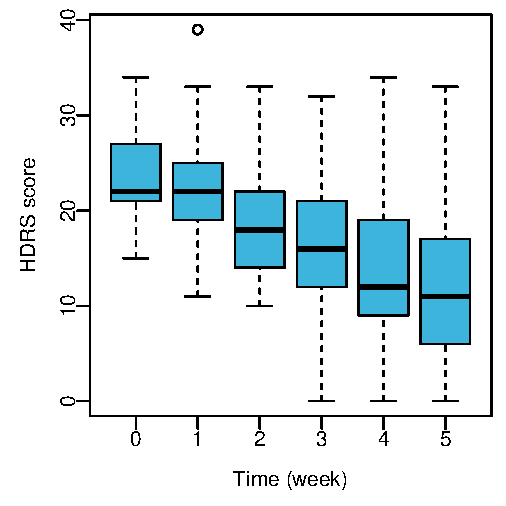
\includegraphics[scale=.8]{fig/hdrs-box}
\end{column}
\begin{column}{.6\textwidth}
  HDRS score\\[1ex]
  {\footnotesize
\begin{tabular}{rrrrrrr}
  \hline
  $t$ & W0 & W1 & W2 & W3 & W4 & W5 \\ 
  \hline
  $M$  & 23.44 & 21.84 & 18.31 & 16.42 & 13.62 & 11.95 \\ 
  $SD$ &  4.53 & 4.70  & 5.49  & 6.42  & 6.97  & 7.22 \\ 
  $n$  & 61    & 63    & 65    & 65    & 63    & 58    \\ 
  \hline
\end{tabular}
  }

  \vspace{.5cm}
  Empirical correlation matrix of HDRS score\\[1ex]
  {\footnotesize
\begin{tabular}{rrrrrrr}
  \hline
   & W0 & W1 & W2 & W3 & W4 & W5 \\ 
  \hline
  Week 0 &   1 & .49 & .41 & .33 & .23 & .18 \\ 
  Week 1 & .49 &   1 & .49 & .41 & .31 & .22 \\ 
  Week 2 & .41 & .49 &   1 & .74 & .67 & .46 \\ 
  Week 3 & .33 & .41 & .74 &   1 & .82 & .57 \\ 
  Week 4 & .23 & .31 & .67 & .82 &   1 & .65 \\ 
  Week 5 & .18 & .22 & .46 & .57 & .65 &   1 \\ 
  \hline
\end{tabular}
  }

  \vspace{1cm}
\end{column}
\end{columns}
\end{frame}

\begin{frame}[fragile]{Depression and Imipramin}
  \begin{lstlisting}
dat      <- read.table("data/reisby.dat", header = TRUE)
dat$id   <- factor(dat$id)
dat$diag <- factor(dat$diag, levels = c("nonen", "endog"))
dat      <- na.omit(dat)     # drop missing values

# descriptive statistics
aggregate(hamd ~ week, dat, mean)
aggregate(hamd ~ week, dat, sd)
aggregate(hamd ~ week, dat, length)
dat[, c("hamd", "id", "week")] |>
  reshape(direction = "wide", timevar = "week") |>
  dplyr::select(-id) |>
  cor(use = "pairwise.complete.obs") |>
  round(3)
  \end{lstlisting}
\end{frame}


\begin{frame}{Depression and Imipramin -- individual processes}
  \vspace{-.2cm}
  \begin{center}
    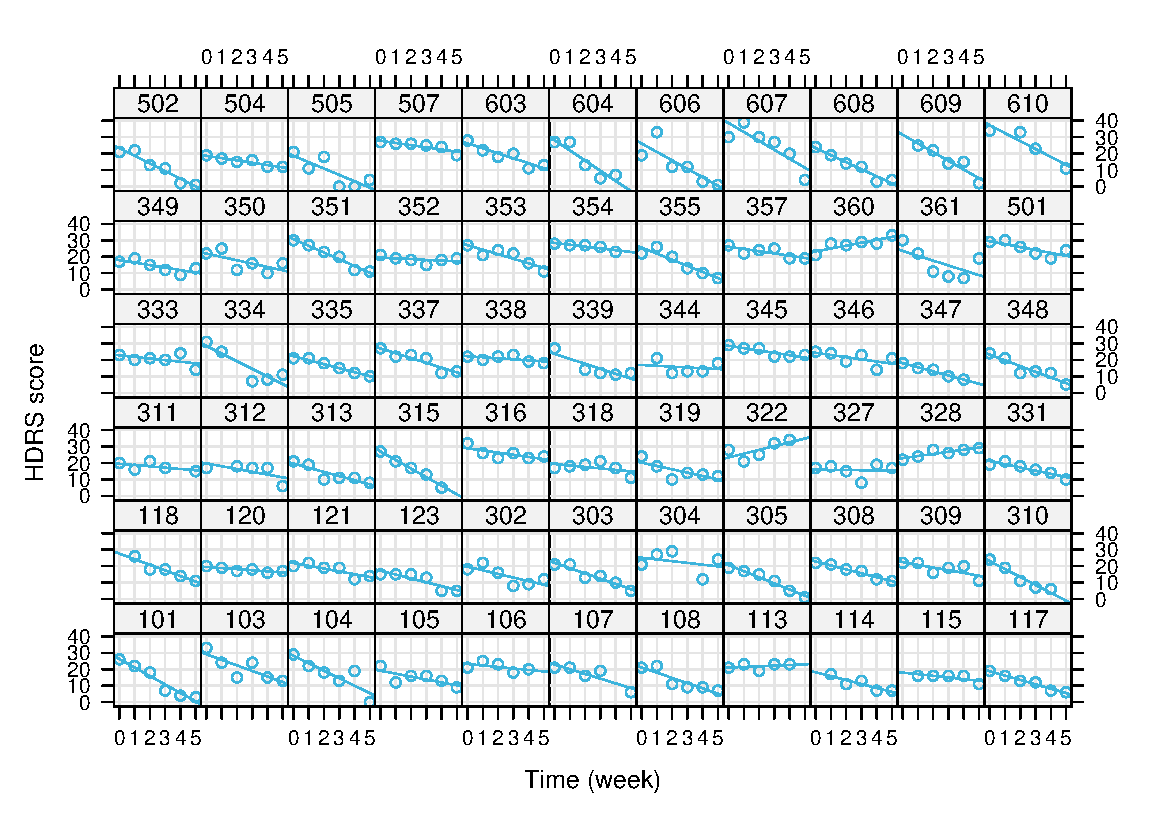
\includegraphics[width = 11cm]{fig/hdrs-ind}
  \end{center}
\end{frame}

\begin{frame}{Alternative model with a constant time term}
  \centering
  \vspace{-1cm}
  \[
    y_{ij} = \beta_0 + \beta_1 time + \upsilon_{0i} + \varepsilon_{ij}
  \]
with $\upsilon_{0i} \sim N(0, \sigma^2_{\upsilon})$ i.i.d.,
$\varepsilon_{ij} \sim N(0, \sigma^2)$ i.i.d., $\upsilon_{0i}$ and
$\varepsilon_{ij}$ i.i.d.\\[2ex]
%  with $\varepsilon_{ij} \sim N(0, \sigma_{\varepsilon}^2)$ i.i.d.\ and
%  $\upsilon_{0i} \sim N(0, \sigma_{\upsilon})$ i.i.d.\\~\\

  \begin{tabular}{cccccc}
    \hline
    response & intercept & time effect & time & subject effect  & residual \\
    \hline
    $y_{11}$ & $\beta_0$ & $\beta_1$   & 0    & $\upsilon_{1}$ & $\varepsilon_{11}$ \\
    $y_{12}$ & $\beta_0$ & $\beta_1$   & 1    & $\upsilon_{1}$ & $\varepsilon_{12}$ \\
    $y_{13}$ & $\beta_0$ & $\beta_1$   & 2    & $\upsilon_{1}$ & $\varepsilon_{13}$ \\
    \vdots & \vdots & \vdots   & \vdots & \vdots & \vdots \\
    $y_{21}$ & $\beta_0$ & $\beta_1$   & 0    & $\upsilon_{2}$ & $\varepsilon_{21}$ \\
    $y_{22}$ & $\beta_0$ & $\beta_1$   & 1    & $\upsilon_{2}$ & $\varepsilon_{22}$ \\
    $y_{23}$ & $\beta_0$ & $\beta_1$   & 2    & $\upsilon_{2}$ & $\varepsilon_{23}$ \\
    \vdots & \vdots & \vdots   & \vdots & \vdots & \vdots \\
    $y_{Nn}$ & $\beta_0$ & $\beta_1$   & n    & $\upsilon_{N}$ & $\varepsilon_{Nn}$ \\
    \hline
  \end{tabular}
\end{frame}

\begin{frame}[fragile]{Random intercept model}
  \[
    y_{ij} = \beta_0 + \beta_1 time + \upsilon_{0i} + \varepsilon_{ij}
  \]
with $\upsilon_{0i} \sim N(0, \sigma^2_{\upsilon})$ i.i.d.,
$\varepsilon_{ij} \sim N(0, \sigma^2)$ i.i.d., $\upsilon_{0i}$ and
$\varepsilon_{ij}$ i.i.d.\\[2ex]
\begin{columns}
\begin{column}{.4\textwidth}
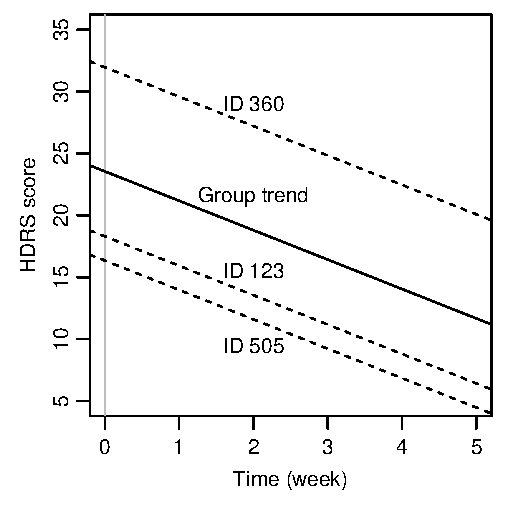
\includegraphics[width=5.5cm]{fig/hdrs-lme1}
\end{column}
%
\begin{column}{.5\textwidth}
  \begin{itemize}
    \item The estimated mean baseline HDRS score is $\hat{\beta}_0 =
      23.55$
    \item However, the estimated standard deviation between patients is
      $\hat{\sigma}_\upsilon = 4.02$
    \item The mean improvement per week is $\hat{\beta}_1 = -2.38$
  \end{itemize}
  \vspace{1cm}
\end{column}
\end{columns}
\end{frame}

\begin{frame}{Implied marginal covariance matrix}
  \begin{itemize}
    \item For the three time points $t_{ij} = 0, 1, 2$, $\mat{Z}_i =
      \vect{1}'_{n_i}$ and $\gmat{\Sigma}_\upsilon = \sigma^2_\upsilon$ we
      get
\begin{align*}
  Cov(\vect{y}_i) &=
    \mat{Z}_i \gmat{\Sigma}_\upsilon \mat{Z}'_i + \sigma^2 \mat{I}_{n_i} \\
  &= \sigma^2_\upsilon \vect{1}_{n_i} \vect{1}'_{n_i} +
     \sigma^2 \mat{I}_{n_i} \\
  &= 
  \begin{pmatrix}
    \sigma^2_\upsilon + \sigma^2 & \sigma^2_\upsilon & \sigma^2_\upsilon \\
    \sigma^2_\upsilon & \sigma^2_\upsilon + \sigma^2 & \sigma^2_\upsilon \\
    \sigma^2_\upsilon & \sigma^2_\upsilon & \sigma^2_\upsilon + \sigma^2
  \end{pmatrix}
\end{align*}
\item The random intercept model implies the compound symmetry structure
  \end{itemize}
\end{frame}

\begin{frame}[fragile]{Random slope model}
  \[
    y_{ij} = \beta_0 + \beta_1 time + \upsilon_{0i} + \upsilon_{1i} time +
    \varepsilon_{ij}
  \]
with
\begin{align*}
  \begin{pmatrix} \upsilon_{0i}\\ \upsilon_{1i} \end{pmatrix} &\sim
    N \left(\begin{pmatrix} 0\\ 0 \end{pmatrix}, \, \gmat{\Sigma}_\upsilon =
      \begin{pmatrix}
        \sigma^2_{\upsilon_0} & \sigma_{\upsilon_0 \upsilon_1} \\
        \sigma_{\upsilon_0 \upsilon_1} & \sigma^2_{\upsilon_1} \\
      \end{pmatrix} \right)
    \text{ i.i.d.} \\
  \gvect{\varepsilon}_i &\sim N(\vect{0}, \, \sigma^2 \mat{I}_{n_i})
    \text{ i.i.d.}
\end{align*}
  \begin{itemize}
    \item Individual intercepts and slopes each have a unique variance
      component and correlate with $\varrho_{\upsilon_0 \upsilon_1} =
      \frac{\sigma_{\upsilon_0 \upsilon_1}}{\sigma_{\upsilon_0} \,
      \sigma_{\upsilon_1}}$
  \end{itemize}
\end{frame}

\begin{frame}{Model predictions}
\begin{columns}
  \begin{column}{.4\textwidth}
    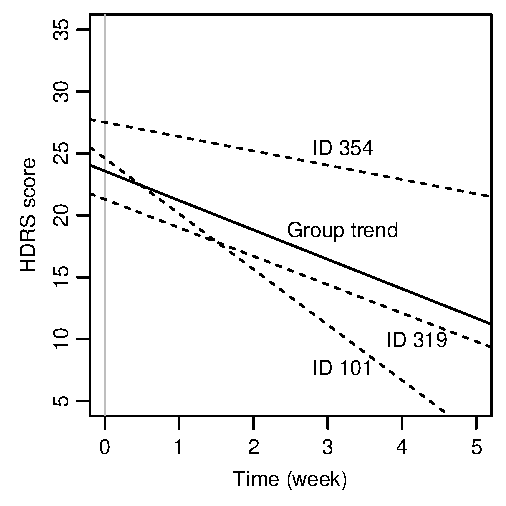
\includegraphics[width=5cm]{fig/hdrs-lme2}
  \end{column}
  \begin{column}{.6\textwidth}
    \begin{itemize}
      \item The estimated mean baseline HDRS score is $\hat{\beta}_0 = 23.58$
      \item The estimated standard deviation between patients is
        $\hat{\sigma}_{\upsilon_0} = 3.55$
      \item The mean improvement per week is $\hat{\beta}_1 = -2.38$
      \item The estimated standard deviation between patients is
        $\hat{\sigma}_{\upsilon_1} = 1.44$
    \end{itemize}
  \end{column}
\end{columns}
  \begin{itemize}
    \item The estimated correlation between individual intercepts and
      slopes is $\hat{\varrho}_{\upsilon_0 \upsilon_1} = -0.28$
    \item Patients with higher (that means worse) baseline scores improve
      more strongly than patients with smaller baseline scores
  \end{itemize}
\end{frame}

\begin{frame}{Implied marginal covariance matrix}
  \begin{itemize}
    \item For the three time points $t_{ij} = 0, 1, 2$,
\[
  \mat{Z}_i =
    \begin{pmatrix}
      1 & 0 \\
      1 & 1 \\
      1 & 2 \\
    \end{pmatrix}
  \text{ und }
  \gmat{\Sigma}_\upsilon =
    \begin{pmatrix}
      \sigma^2_{\upsilon_0} & \sigma_{\upsilon_0 \upsilon_1} \\
      \sigma_{\upsilon_0 \upsilon_1} & \sigma^2_{\upsilon_1}
    \end{pmatrix}
\]
we get
\begin{align*}
  & Cov(\vect{y}_i) =
    \mat{Z}_i \gmat{\Sigma}_\upsilon \mat{Z}'_i + \sigma^2 \mat{I}_{n_i} \\
  &= \begin{pmatrix}
    \sigma^2_{\upsilon_0}                                    & \sigma^2_{\upsilon_0} + \sigma_{\upsilon_0 \upsilon_1}                             & \sigma^2_{\upsilon_0} + 2 \sigma_{\upsilon_0 \upsilon_1} \\
    \sigma^2_{\upsilon_0} + \sigma_{\upsilon_0 \upsilon_1}   & \sigma^2_{\upsilon_0} + 2 \sigma_{\upsilon_0 \upsilon_1} + \sigma^2_{\upsilon_1}   & \sigma^2_{\upsilon_0} + 3 \sigma_{\upsilon_0 \upsilon_1} + 2 \sigma^2_{\upsilon_1} \\
    \sigma^2_{\upsilon_0} + 2 \sigma_{\upsilon_0 \upsilon_1} & \sigma^2_{\upsilon_0} + 3 \sigma_{\upsilon_0 \upsilon_1} + 2 \sigma^2_{\upsilon_1} & \sigma^2_{\upsilon_0} + 4 \sigma_{\upsilon_0 \upsilon_1} + 4 \sigma^2_{\upsilon_1} \\
  \end{pmatrix}
   + \sigma^2 \mat{I}_{n_i}
\end{align*}
\item Hence, a more flexible covariance structure when compared to compound
  symmetry
  \end{itemize}
\end{frame}

\begin{frame}[fragile]{Fitting mixed-effects models}
\begin{lstlisting}
# random intercept model
lme1 <- lmer(hamd ~ week + (1 | id), dat, REML = FALSE)
summary(lme1)

# random slope model
lme2 <- lmer(hamd ~ week + (week | id), dat, REML = FALSE)
summary(lme2)

# model comparison
anova(lme1, lme2)
\end{lstlisting}
\end{frame}
 
% TODO: Go over slides for Reisby and descide what you need (and if any!)

\begin{frame}[fragile]{Means and predicted HDRS score by group}
  \begin{lstlisting}

dat2 <- aggregate(hamd ~ week + diag, dat, mean)
dat2$m4 <- predict(m4, newdata = dat2, re.form = ~ 0)

plot(m4 ~ week, dat2[dat2$diag == "endog", ], type = "l",
     ylim=c(0, 28), xlab="Week", ylab = "HDRS score")
lines(m4 ~ week, dat2[dat2$diag == "nonen", ], lty = 2)
points(hamd ~ week, dat2[dat2$diag == "endog", ], pch = 16)
points(hamd ~ week, dat2[dat2$diag == "nonen", ], pch = 21, bg = "white")
legend("topright", c("Endogenous", "Non endogenous"),
       lty = 1:2, pch = c(16, 21), pt.bg = "white", bty = "n")

  \end{lstlisting}
\end{frame}

\begin{frame}[fragile]{Gory details}
  \begin{lstlisting}
fixef(m4)
getME(m4, "theta")
t(chol(VarCorr(m4)$id))[lower.tri(diag(2), diag = TRUE)] / sigma(m4)
  \end{lstlisting}
\end{frame}

\begin{frame}[fragile]{Power simulation}
  \begin{lstlisting}
## Study design and sample sizes
n_week <- 6
n_subj <- 80
n <- n_week * n_subj
dat <- data.frame(
     id = rep(seq_len(n_subj), each = n_week),
   week = rep(0:(n_week - 1), times = n_subj),
  treat = rep(0:1, each = n/2)
)
  \end{lstlisting}
\end{frame}

\begin{frame}[fragile]{Power simulation}
  \begin{lstlisting}
## Fixed effects and variance components
beta <- c("(Intercept)" = 23, week = -0.5, treat = 0, "week:treat" = -1)
s <- 3.5                # residual sd
r <- -0.3
t(chol(VarCorr(m4)$id))[lower.tri(diag(2), diag = TRUE)] / sigma(m3)
# su <- c(3.5, 1.5)
# Su <- r * su %o% su
# diag(Su) <- su^2        # covariance matrix of random effects

su1 <- 3.5
su2 <- 1.5
Su <- matrix(c(su1^2, r * su1 * su2, r * su1 * su2, su2^2), nrow = 2, ncol = 2)

Lt <- chol(Su) / s
pars <- list(theta = t(Lt)[lower.tri(Lt, TRUE)],
             beta = beta, sigma = s)
names(pars$theta) <- c("id.(Intercept)", "id.week.(Intercept)", "id.week")
  \end{lstlisting}
\end{frame}

\begin{frame}[fragile]{Power simulation}
  \begin{lstlisting}
## Power
pval <- replicate(200, {
  y <- simulate(~ week * treat + (week | id),
                newparams = pars, newdata = dat)$sim_1
  m1 <- lmer(y ~ week + treat + (week | id), data = dat, REML = FALSE)
  m2 <- lmer(y ~ week * treat + (week | id), data = dat, REML = FALSE)
  anova(m1, m2)$"Pr(>Chisq)"[2]
})

mean(pval < 0.05)
  \end{lstlisting}
\end{frame}

\begin{frame}[fragile]{Power simulation}
  \begin{lstlisting}
## Parameter recovery
y <- simulate(~ week * treat + (week | id),
              newparams = pars, newdata = dat)$sim_1
m <- lmer(y ~ week * treat + (week | id), data = dat, REML = FALSE)
fixef(m)
VarCorr(m)
  \end{lstlisting}
\end{frame}

\appendix
\begin{frame}{References}
%\begin{frame}[allowframebreaks]{References}
%\renewcommand{\bibfont}{\footnotesize}
\bibliographystyle{apacite}
\bibliography{../lit}
\end{frame}

\end{document}

